\part{\Exercises{}}

\clearpage
\begin{center}
\vspace*{\fill}

\begin{figure}[H]
\centering
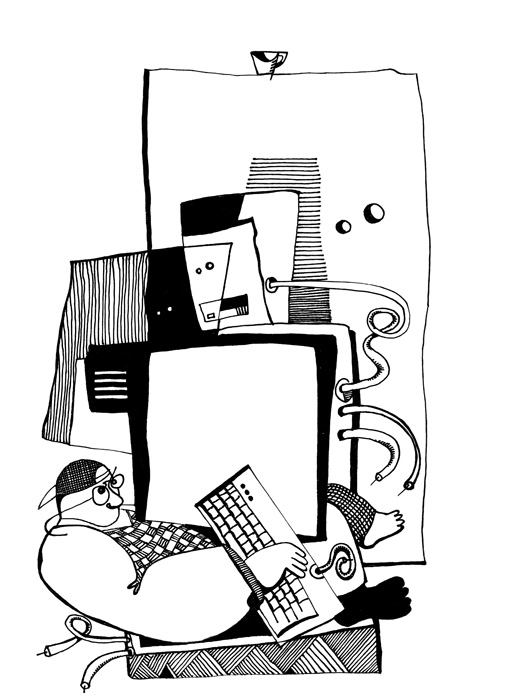
\includegraphics[scale=\FigScale]{cover3.jpg}
\end{figure}

\vspace*{\fill}
\end{center}

\clearpage

\RU{Почти для всех задач, если не указано иное, два вопроса:}
\EN{There are two questions almost for every exercise, if otherwise not specified:}

1) \RU{Что делает эта функция? Ответ должен состоять из одной фразы.}
\EN{What does this function do? Answer in one sentence.}

2) \RU{Перепишите эту функцию на \CCpp}\EN{Rewrite this function into \CCpp}.

\RU{Пользоваться Google-м, для поиска
каких-либо зацепок, разрешается}\EN{It is allowed to use Google to search for any leads}.
\RU{Впрочем, для усложнения своей задачи, вы можете попробовать и без Google}
\EN{However, if you like to make your task harder, you may try to solve it without using Google}.

\RU{Подсказки и ответы собраны в приложении к этой книге.}\EN{Some hints and the solutions can be found in the appendix of
this book.}

\chapter{\IFRU{Уровень}{Level} 1}

\IFRU{Задачи первого уровня, это те, которые можно решать голове}{Level 1 exercises are ones you
may try to solve in mind}.

\section{\Exercise 1.1}
% max()

\subsection{MSVC 2012 x64 + \Ox}

\index{x86!\Instructions!CMOVcc}
\begin{lstlisting}
a$ = 8
b$ = 16
f	PROC
	cmp	ecx, edx
	cmovg	edx, ecx
	mov	eax, edx
	ret	0
f	ENDP
\end{lstlisting}

\subsection{Keil (ARM)}

\begin{lstlisting}
        CMP      r0,r1
        MOVLE    r0,r1
        BX       lr
\end{lstlisting}

\subsection{Keil (thumb)}
        
\begin{lstlisting}
	CMP      r0,r1
        BGT      |L0.6|
        MOVS     r0,r1
|L0.6|
        BX       lr
\end{lstlisting}

\section{\Exercise 1.2}

\index{x86!\Instructions!LOOP}
\IFRU{Почему инструкция}{Why} \LOOP \IFRU{больше не используется компиляторами}{instruction is 
not used by compilers anymore}?

\section{\Exercise 1.3}

\IFRU{Возьмите пример из секции}{Take an loop example from} ``\Loops''\EN{ section} (\ref{sec:loops}), 
\IFRU{скомпилируйте его в вашей любимой}{compile it in your favorite} \ac{OS}
\IFRU{и компиляторе, и модифицируйте исполняемый файл так, чтобы цикл был в пределах}{and compiler 
and modify (patch) executable file, so the loop range will be} [6..20].


\chapter{\RU{Уровень}\EN{Level} 2}

\RU{Для решения задач второго уровня, вам вероятно понадобится текстовый редактор или тетрадка с ручкой}
\EN{For solving exercises of level 2, you probably will need text editor or paper and pencil}.

\section{\Exercise 2.1}
% sqrt

\subsection{\Optimizing MSVC 2010 x86}

\lstinputlisting{exercises/2/sqrt_MSVC2010_Ox.asm}

\subsection{\Optimizing MSVC 2012 x64}

\lstinputlisting{exercises/2/sqrt_MSVC2012_Ox_x64.asm}

% 2.2
% 2.3

\section{\Exercise 2.4}
% strstr()

\RU{Это стандартная функция из библиотек Си. Исходник взят из MSVC 2010.}
\EN{This is standard C library function. Source code taken from MSVC 2010.}

\subsection{\Optimizing MSVC 2010}

\lstinputlisting{exercises/1_4_msvc.asm}

\subsection{GCC 4.4.1}

\lstinputlisting{exercises/1_4_gcc.asm}

\subsection{\Optimizing Keil (\ARMMode)}

\lstinputlisting{exercises/1_4_ARM.s}

\subsection{\Optimizing Keil (\ThumbMode)}

\lstinputlisting{exercises/1_4_thumb.s}

\subsection{\Optimizing GCC 4.9.1 (ARM64)}

\lstinputlisting[caption=\Optimizing GCC 4.9.1 (ARM64)]{exercises/1_4_ARM64_O3.s}

\subsection{\Optimizing GCC 4.4.5 (MIPS)}

\lstinputlisting[caption=\Optimizing GCC 4.4.5 (MIPS) (IDA)]{exercises/1_4_MIPS_O3_IDA.lst}

% 2.5

\section{\Exercise 2.6}
% TEA

\subsection{\Optimizing MSVC 2010}

\lstinputlisting{exercises/1_6_msvc.asm}

\subsection{\Optimizing Keil (\ARMMode)}

\lstinputlisting{exercises/1_6_ARM.s}

\subsection{\Optimizing Keil (\ThumbMode)}

\lstinputlisting{exercises/1_6_thumb.s}

\subsection{\Optimizing GCC 4.9.1 (ARM64)}

\lstinputlisting[caption=\Optimizing GCC 4.9.1 (ARM64)]{exercises/1_6_ARM64_O3.s}

\subsection{\Optimizing GCC 4.4.5 (MIPS)}

\lstinputlisting[caption=\Optimizing GCC 4.4.5 (MIPS) (IDA)]{exercises/1_6_MIPS_O3_IDA.lst}

% 2.7
% 2.8
% 2.9
% 2.10
% 2.11
% 2.12

\section{\Exercise 2.13}
% LFSR

\RU{Это довольно известный криптоалгоритм прошлого}\EN{This is a well-known cryptoalgorithm of the past}.
\RU{Как он называется}\EN{How it's called}?

\subsection{\Optimizing MSVC 2012}

\begin{lstlisting}
_in$ = 8						; size = 2
_f	PROC
	movzx	ecx, WORD PTR _in$[esp-4]
	lea	eax, DWORD PTR [ecx*4]
	xor	eax, ecx
	add	eax, eax
	xor	eax, ecx
	shl	eax, 2
	xor	eax, ecx
	and	eax, 32					; 00000020H
	shl	eax, 10					; 0000000aH
	shr	ecx, 1
	or	eax, ecx
	ret	0
_f	ENDP
\end{lstlisting}

\subsection{Keil (\ARMMode)}

\begin{lstlisting}
f PROC
        EOR      r1,r0,r0,LSR #2
        EOR      r1,r1,r0,LSR #3
        EOR      r1,r1,r0,LSR #5
        AND      r1,r1,#1
        LSR      r0,r0,#1
        ORR      r0,r0,r1,LSL #15
        BX       lr
        ENDP
\end{lstlisting}

\subsection{Keil (\ThumbMode)}

\begin{lstlisting}
f PROC
        LSRS     r1,r0,#2
        EORS     r1,r1,r0
        LSRS     r2,r0,#3
        EORS     r1,r1,r2
        LSRS     r2,r0,#5
        EORS     r1,r1,r2
        LSLS     r1,r1,#31
        LSRS     r0,r0,#1
        LSRS     r1,r1,#16
        ORRS     r0,r0,r1
        BX       lr
        ENDP
\end{lstlisting}

\subsection{\Optimizing GCC 4.9.1 (ARM64)}

\begin{lstlisting}
f:
	uxth	w1, w0
	lsr	w2, w1, 3
	lsr	w0, w1, 1
	eor	w2, w2, w1, lsr 2
	eor	w2, w1, w2
	eor	w1, w2, w1, lsr 5
	and	w1, w1, 1
	orr	w0, w0, w1, lsl 15
	ret
\end{lstlisting}

\subsection{\Optimizing GCC 4.4.5 (MIPS)}

\lstinputlisting[caption=\Optimizing GCC 4.4.5 (MIPS) (IDA)]{exercises/2_13_MIPS_O3_IDA.lst}

\section{\Exercise 2.14}
% GCD

\RU{Еще один хорошо известный алгоритм. Ф-ция берет на вход 2 значения и возвращает одно.}
\EN{Another well-known algorithm. The function takes two variables and returning one.}

\subsection{MSVC 2012}

\index{x86!\Instructions!BSF}
\lstinputlisting{exercises/2/GCD_MSVC_2012_Ox.asm}

\subsection{Keil (\ARMMode)}

\index{ARM!\Instructions!CLZ}
\lstinputlisting{exercises/2/GCD_Keil_ARM_O3.s}

\subsection{GCC 4.6.3 for Raspberry Pi (\ARMMode)}

\index{ARM!\Instructions!CLZ}
\lstinputlisting{exercises/2/GCD_ARM_pi_GCC_4.6.3_O3.s}

\subsection{\Optimizing GCC 4.9.1 (ARM64)}

\lstinputlisting[caption=\Optimizing GCC 4.9.1 (ARM64)]{exercises/2/GCD_ARM64_GCC491_O3.s}

\subsection{\Optimizing GCC 4.4.5 (MIPS)}

\lstinputlisting[caption=\Optimizing GCC 4.4.5 (MIPS) (IDA)]{exercises/2/GCD_MIPS_O3_IDA.lst}

\section{\Exercise 2.15}
% Monte Carlo

\RU{И снова известный алгоритм. Что он делает?}\EN{Well-known algorithm again. What it does?}

\RU{Обратите внимание, что код для x86 использует FPU, а для x64 --- SIMD-инструкции. Это нормально}
\EN{Take also notice that the code for x86 uses FPU, but SIMD-instructions are used instead in x64 code.
That's OK}: \myref{floating_SIMD}.

\subsection{\Optimizing MSVC 2012 x64}

\lstinputlisting{exercises/2/monte_MSVC_2012_Ox_x64.asm}

\subsection{\Optimizing GCC 4.4.6 x64}

\lstinputlisting{exercises/2/monte_GCC_4.4.6_O3_x64.s}

\subsection{\Optimizing GCC 4.8.1 x86}

\lstinputlisting{exercises/2/monte_GCC_4.8.1_O3_x86.s}

\subsection{Keil (\ARMMode): \RU{для процессора Cortex-R4F}\EN{Cortex-R4F CPU as target}}

\lstinputlisting{exercises/2/monte_Keil_ARM_Cortex.s}

\subsection{\Optimizing GCC 4.9.1 (ARM64)}

\lstinputlisting[caption=\Optimizing GCC 4.9.1 (ARM64)]{exercises/2/monte_GCC_491_ARM64_O3.s}

\subsection{\Optimizing GCC 4.4.5 (MIPS)}

\lstinputlisting[caption=\Optimizing GCC 4.4.5 (MIPS) (IDA)]{exercises/2/monte_GCC_4.4.6_O3_x64.s}

\section{\Exercise 2.16}
% Ackermann function

\RU{Известная функция. Что она вычисляет? Почему стек переполняется если на вход подать
числа 4 и 2? Есть ли здесь какая-то ошибка?}\EN{Well-known function. What it computes? 
Why stack overflows if 4 and 2 are supplied at input? Are there any error?}

\subsection{\Optimizing MSVC 2012 x64}

\lstinputlisting{exercises/2/ack_MSVC_Ox_x64.asm}

\subsection{\Optimizing Keil (\ARMMode)}

\lstinputlisting{exercises/2/ack_ARM_O3.s}

\subsection{\Optimizing Keil (\ThumbMode)}

\lstinputlisting{exercises/2/ack_thumb_O3.s}

\subsection{\NonOptimizing GCC 4.9.1 (ARM64)}

\lstinputlisting[caption=\NonOptimizing GCC 4.9.1 (ARM64)]{exercises/2/ack_ARM64_GCC491_O0.s}

\subsection{\Optimizing GCC 4.9.1 (ARM64)}

\RU{Оптимизирующий GCC генерирует куда больше кода. Почему?}
\EN{Optimizing GCC generates much more code. Why?}

\lstinputlisting[caption=\Optimizing GCC 4.9.1 (ARM64)]{exercises/2/ack_ARM64_GCC491_O3.s}

\subsection{\NonOptimizing GCC 4.4.5 (MIPS)}

\lstinputlisting[caption=\NonOptimizing GCC 4.4.5 (MIPS) (IDA)]{exercises/2/ack_MIPS_O0_IDA.lst}

\section{\Exercise 2.17}
% Rule 110

\RU{Эта программа выдает в \gls{stdout} какую-то информацию, каждый раз --- разную}\EN{This program
prints some information to \gls{stdout}, each time different}.
\RU{Что это}\EN{What is it}?

\RU{Скомпилированные бинарные файлы}\EN{Compiled binaries}:

\begin{itemize}
\item \href{http://go.yurichev.com/17170}{Linux x64 (beginners.re)}
\item \href{http://go.yurichev.com/17171}{\MacOSX (beginners.re)}
\item \href{http://go.yurichev.com/17172}{Linux MIPS (beginners.re)}
\item \href{http://go.yurichev.com/17173}{Win32 (beginners.re)}
\item \href{http://go.yurichev.com/17174}{Win64 (beginners.re)}
\end{itemize}

\RU{Для версий под Windows, возможно, нужно будет установить}
\EN{As of Windows versions, you may need to install} 
\href{http://go.yurichev.com/17302}{MSVC 2012 redist}.

\section{\Exercise 2.18}

\RU{Эта программа запрашивает пароль}\EN{This program requires password}.
\RU{Найдите его}\EN{Find it}.

\RU{Кстати, не только один пароль может подойти}\EN{By the way, multiple passwords may work}. 
\RU{Попробуйте найти еще}\EN{Try to find more}.

\RU{Как дополнительное упражнение, попробуйте изменить пароль модифицируя исполняемый файл}
\EN{As an additional exercise, try to change the password by patching executable file}.

\begin{itemize}
\item \href{http://go.yurichev.com/17175}{Win32 (beginners.re)}
\item \href{http://go.yurichev.com/17176}{Linux x86 (beginners.re)}
\item \href{http://go.yurichev.com/17177}{\MacOSX (beginners.re)}
\item \href{http://go.yurichev.com/17178}{Linux MIPS (beginners.re)}
\end{itemize}

\section{\Exercise 2.19}

\RU{То же что и в упражнении}\EN{The same as in exercise} 2.18.

\begin{itemize}
\item \href{http://go.yurichev.com/17179}{Win32 (beginners.re)}
\item \href{http://go.yurichev.com/17180}{Linux x86 (beginners.re)}
\item \href{http://go.yurichev.com/17181}{\MacOSX (beginners.re)}
\item \href{http://go.yurichev.com/17182}{Linux MIPS (beginners.re)}
\end{itemize}

\section{\Exercise 2.20}
% Collatz conjecture

\RU{Эта программа выдает в \gls{stdout} какие-то числа.}
\EN{This program prints some numbers to \gls{stdout}.}
\RU{Что это}\EN{What is it}?

\RU{Скомпилированные бинарные файлы}\EN{Compiled binaries}:

\begin{itemize}
\item \href{http://go.yurichev.com/17183}{Linux x64 (beginners.re)}
\item \href{http://go.yurichev.com/17184}{\MacOSX (beginners.re)}
\item \href{http://go.yurichev.com/17185}{Linux ARM Raspberry Pi (beginners.re)}
\item \href{http://go.yurichev.com/17186}{Linux MIPS (beginners.re)}
\item \href{http://go.yurichev.com/17187}{Win64 (beginners.re)}
\end{itemize}

\chapter{\RU{Уровень}\EN{Level} 3}

\RU{Для решения задач третьего уровня вам придется потратить какое-то ощутимое время, 
вплоть до одного дня}
\EN{For solving level 3 tasks, you'll probably need considerable amount of time, maybe up to one day}.

% 3.1

\section{\Exercise 3.2}

\RU{Имеется небольшой исполняемый файл, внутри которого находится довольно известная криптосистема}
\EN{There is a small executable file with a well-known cryptosystem inside}.
\RU{Попробуйте её идентифицировать}\EN{Try to identify it}.

\begin{itemize}
\item \href{http://go.yurichev.com/17188}{Windows x86}
\item \href{http://go.yurichev.com/17189}{Linux x86}
\item \href{http://go.yurichev.com/17190}{\MacOSX (x64)}
\item \href{http://go.yurichev.com/17191}{Linux MIPS}
\end{itemize}

\section{\Exercise 3.3}
% entropy

\RU{Имеется небольшой исполняемый файл, некая утилита}
\EN{There is a small executable file, some utility}.
\RU{Она открывает другой файл, читает его, что-то вычисляет и показывает число с плавающей точкой}
\EN{It opens another file, reads it, calculate something and prints a float number}.
\RU{Попробуйте разобраться, что она делает}\EN{Try to understand what it do}.

\begin{itemize}
\item \href{http://go.yurichev.com/17192}{Windows x86}
\item \href{http://go.yurichev.com/17193}{Linux x86}
\item \href{http://go.yurichev.com/17194}{\MacOSX (x64)}
\item \href{http://go.yurichev.com/17195}{Linux MIPS}
\end{itemize}

\section{\Exercise 3.4}

\RU{Утилита, шифрующая и дешифрующая файлы, по паролю}
\EN{There is an utility which encrypts/decrypts files, by password}.
\RU{Есть зашифрованный текстовый файл, пароль неизвестен}\EN{There is an encrypted text file,
password is unknown}.
\RU{Зашифрованный файл ~--- это текст на английском языке}\EN{Encrypted file is a text in English language}.
\RU{Утилита использует сравнительно мощный алгоритм шифрования, тем не менее,
он был применен с очень грубой ошибкой. И из-за ошибки расшифровать файл вполне возможно 
с минимумом затрат.}
\EN{The utility uses relatively strong cryptosystem, nevertheless, it was implemented with a serious blunder.
Since the mistake present, it is possible to decrypt the file with a little effort.}

\RU{Попробуйте найти ошибку и расшифровать файл}\EN{Try to find the mistake and decrypt the file}.

\begin{itemize}
\item \href{http://go.yurichev.com/17196}{Windows x86}

\item {\RU{Текстовый файл}\EN{Text file}}: \url{http://go.yurichev.com/17197}
\end{itemize}

\section{\Exercise 3.5}

\RU{Это имитация защиты от копирования использующей ключевой файл}
\EN{This is software copy protection imitation, which uses key file}.
\RU{В ключевом файле имя пользователя и серийный номер}
\EN{The key file contain user (or customer) name and serial number}.

\RU{Задачи две}\EN{There are two tasks}:

\index{tracer}
\begin{itemize}
\item
\RU{(Простая) при помощи \tracer либо иного отладчика, 
заставьте эту программу принимать измененный ключевой файл}\EN{(Easy) with the help of \tracer
or any other debugger, force the program to accept changed key file}.

\item
\RU{(Средняя) ваша задача заключается в том, чтобы изменить в файле имя пользователя на другое, 
но при этом, модифицировать саму программу нельзя}
\EN{(Medium) your goal is to modify user name to another, however, it is not allowed to patch the program}.
\end{itemize}

\begin{itemize}
\item \href{http://go.yurichev.com/17198}{Windows x86}
\item \href{http://go.yurichev.com/17199}{Linux x86}
\item \href{http://go.yurichev.com/17200}{\MacOSX (x64)}
\item \href{http://go.yurichev.com/17201}{Linux MIPS}
\item \RU{Ключевой файл}\EN{Key file}: \url{http://go.yurichev.com/17202}
\end{itemize}

\section{\Exercise 3.6}

\RU{Это очень примитивный игрушечный веб-сервер, поддерживающий только статические файлы, без \ac{CGI}, и т.д}
\EN{Here is a very primitive toy web-server, supporting only static files, without \ac{CGI}, etc}.
\RU{В нем сознательно оставлено по крайней мере 4 уязвимости}
\EN{At least 4 vulnerabilities are left here intentionally}.
\RU{Постарайтесь найти их все и использовать для взлома удаленной машины}
\EN{Try to find them all and exploit them in order for breaking into a remote host}.

\begin{itemize}
\item \href{http://go.yurichev.com/17203}{Windows x86}
\item \href{http://go.yurichev.com/17204}{Linux x86}
\item \href{http://go.yurichev.com/17205}{\MacOSX (x64)}
\end{itemize}
% FIXME: MIPS?

% 3.7

\section{\Exercise 3.8}

\RU{Это достаточно известный алгоритм компрессии данных}\EN{It's a well known data compression algorithm}.
\RU{Но из-за ошибки (или даже опечатки) он разжимает неверно}\EN{However, due to mistake (or typo), 
it decompress incorrectly}.
\RU{В этом можно убедиться на этих примерах}\EN{Here we can see this bug in these examples}.\\
\RU{Это исходный текст}\EN{This is a text used as a source}: 
\url{http://go.yurichev.com/17206}\\
\RU{Это корректно сжатый текст}\EN{This is a text compressed correctly}: 
\url{http://go.yurichev.com/17207}\\
\RU{Это некорректно разжатый текст}\EN{This is incorrectly uncompressed text}:
\url{http://go.yurichev.com/17208}.\\
\\
\RU{Попробуйте найти и исправить ошибку}\EN{Try to find and fix bug}.
\RU{При некотором упорстве, это можно сделать при помощи модификации исполняемого файла}
\EN{With some effort, it can be done even by patching}.

\begin{itemize}
\item \href{http://go.yurichev.com/17209}{Windows x86}
\item \href{http://go.yurichev.com/17210}{Linux x86}
\item \href{http://go.yurichev.com/17211}{\MacOSX (x64)}
\end{itemize}

% FIXME: MIPS?



\chapter{crackme / keygenme}

\RU{Несколько моих \gls{keygenme}:}
\EN{Couple of my \glspl{keygenme}:}

\url{http://go.yurichev.com/17315}

